\documentclass{atistandalonetask}
\usepackage{atistandard}

\begin{document}
  \begin{atiTask}[
    title = Dreiecksschwingung
  ]
	Die Abbildung zeigt die sogenannte Dreieckschwingung
	\begin{figure}[H]
	\centering
	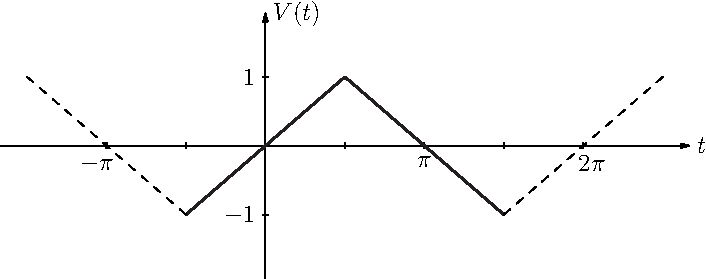
\includegraphics[width=0.7\linewidth]{picture-fourier_iii}
	\caption{Dreiecksschwingung}
	\end{figure}

	\begin{atiSubtasks}
		\item
		Schreiben Sie die Funktion $V(t)$ auf, welche die Dreieckschwingung im Intervall $-\frac{\pi}{2}\leq t\leq \frac{3\pi}{2}$ beschreibt und überzeugen Sie sich, dass die \textsc{Dirichlet}-Bedingungen erfüllt sind.
		\item Entwickeln Sie die Funktion $V(t)$ für den Fall, dass sie sich periodisch wiederholt, in eine \textsc{Fourier}-Reihe. 
		\item Stellen Sie das Spektrum (Koffizienten $a_n$, $b_n$ über $n$) der Dreieckschwingung graphisch dar.
		\item \textbf{Zusatz:} Vergleichen Sie alle Ergebnisse mit den entsprechenden Resultaten für eine Sinusschwingung mit gleicher Amplitude und Periode. 
	\end{atiSubtasks} 
  \end{atiTask}
  \begin{atiSolution}
   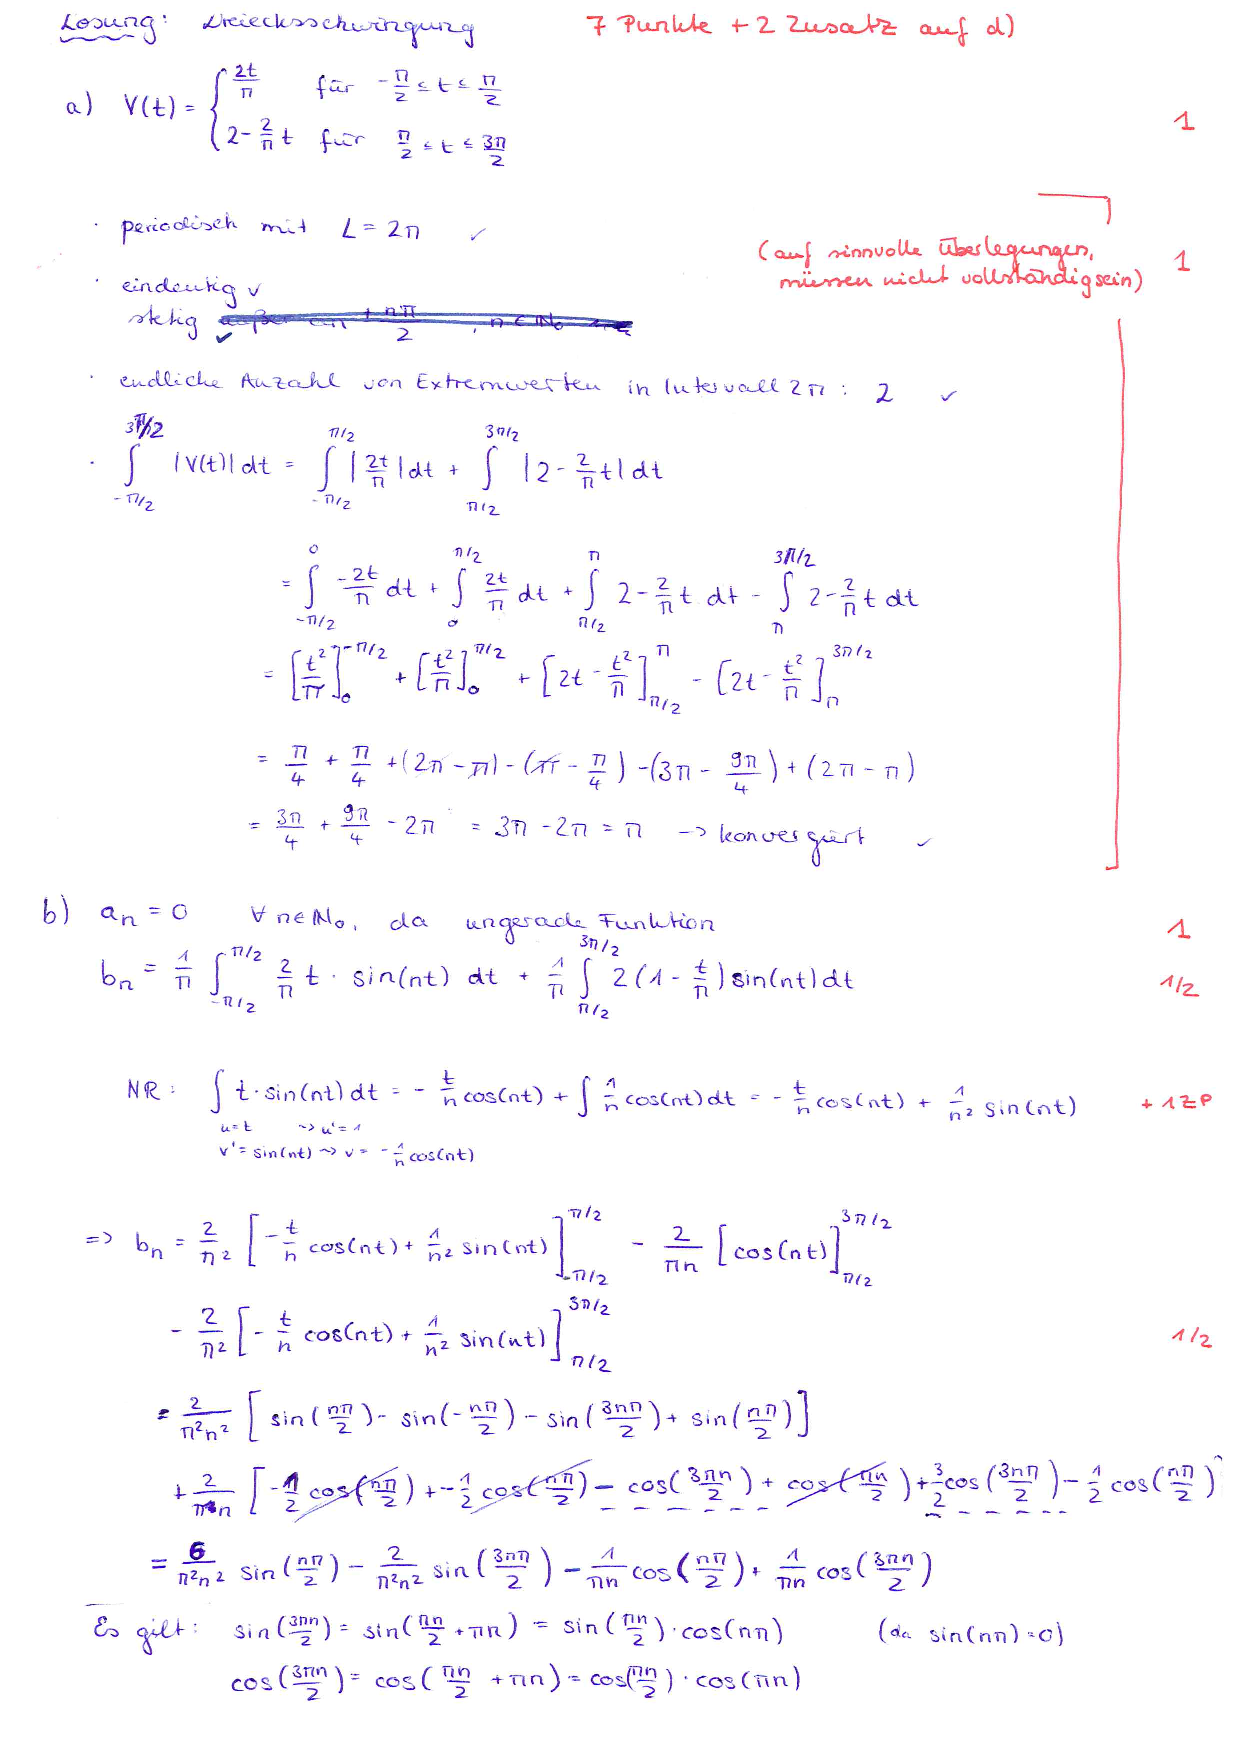
\includepdf[pages=-]{solution-fourier_iii.pdf}
  \end{atiSolution}
\end{document}